\documentclass{article}\usepackage[]{graphicx}\usepackage[]{xcolor}
% maxwidth is the original width if it is less than linewidth
% otherwise use linewidth (to make sure the graphics do not exceed the margin)
\makeatletter
\def\maxwidth{ %
  \ifdim\Gin@nat@width>\linewidth
    \linewidth
  \else
    \Gin@nat@width
  \fi
}
\makeatother

\definecolor{fgcolor}{rgb}{0.345, 0.345, 0.345}
\newcommand{\hlnum}[1]{\textcolor[rgb]{0.686,0.059,0.569}{#1}}%
\newcommand{\hlsng}[1]{\textcolor[rgb]{0.192,0.494,0.8}{#1}}%
\newcommand{\hlcom}[1]{\textcolor[rgb]{0.678,0.584,0.686}{\textit{#1}}}%
\newcommand{\hlopt}[1]{\textcolor[rgb]{0,0,0}{#1}}%
\newcommand{\hldef}[1]{\textcolor[rgb]{0.345,0.345,0.345}{#1}}%
\newcommand{\hlkwa}[1]{\textcolor[rgb]{0.161,0.373,0.58}{\textbf{#1}}}%
\newcommand{\hlkwb}[1]{\textcolor[rgb]{0.69,0.353,0.396}{#1}}%
\newcommand{\hlkwc}[1]{\textcolor[rgb]{0.333,0.667,0.333}{#1}}%
\newcommand{\hlkwd}[1]{\textcolor[rgb]{0.737,0.353,0.396}{\textbf{#1}}}%
\let\hlipl\hlkwb

\usepackage{framed}
\makeatletter
\newenvironment{kframe}{%
 \def\at@end@of@kframe{}%
 \ifinner\ifhmode%
  \def\at@end@of@kframe{\end{minipage}}%
  \begin{minipage}{\columnwidth}%
 \fi\fi%
 \def\FrameCommand##1{\hskip\@totalleftmargin \hskip-\fboxsep
 \colorbox{shadecolor}{##1}\hskip-\fboxsep
     % There is no \\@totalrightmargin, so:
     \hskip-\linewidth \hskip-\@totalleftmargin \hskip\columnwidth}%
 \MakeFramed {\advance\hsize-\width
   \@totalleftmargin\z@ \linewidth\hsize
   \@setminipage}}%
 {\par\unskip\endMakeFramed%
 \at@end@of@kframe}
\makeatother

\definecolor{shadecolor}{rgb}{.97, .97, .97}
\definecolor{messagecolor}{rgb}{0, 0, 0}
\definecolor{warningcolor}{rgb}{1, 0, 1}
\definecolor{errorcolor}{rgb}{1, 0, 0}
\newenvironment{knitrout}{}{} % an empty environment to be redefined in TeX

\usepackage{alltt}
\usepackage{amsmath} %This allows me to use the align functionality.
                     %If you find yourself trying to replicate
                     %something you found online, ensure you're
                     %loading the necessary packages!
\usepackage{amsfonts}%Math font
\usepackage{graphicx}%For including graphics
\usepackage{hyperref}%For Hyperlinks
\usepackage[shortlabels]{enumitem}% For enumerated lists with labels specified
                                  % We had to run tlmgr_install("enumitem") in R
\hypersetup{colorlinks = true,citecolor=black} %set citations to have black (not green) color
\usepackage{natbib}        %For the bibliography
\setlength{\bibsep}{0pt plus 0.3ex}
\bibliographystyle{apalike}%For the bibliography
\usepackage[margin=0.50in]{geometry}
\usepackage{float}
\usepackage{multicol}

%fix for figures
\usepackage{caption}
\newenvironment{Figure}
  {\par\medskip\noindent\minipage{\linewidth}}
  {\endminipage\par\medskip}
\IfFileExists{upquote.sty}{\usepackage{upquote}}{}
\begin{document}

\vspace{-1in}
\title{Lab 7 and 8 -- MATH 240 -- Computational Statistics}

\author{
  Caroline Devine \\
  Colgate University  \\
  Math Department  \\
  {\tt cdevine@colgate.edu}
}

\date{April 1st, 2025}

\maketitle

\begin{multicols}{2}
\begin{abstract}
This lab evaluates and examines the beta distribution seeing how varying parameters affect its shape and statistical properties, focusing on the mean, variance, skewness, and excess kurtosis. Through analyzing real-world data from World Bank, we see the accuracy of how sample estimates approximate the population parameters with different sample sizes and estimators. Our results show that Maximum Likelihood Estimation provides slightly more precise estimates, but both Method of Moments and Maximum Likelihood Estimation are sufficient estimators. 
\end{abstract}

\noindent \textbf{Keywords:} Beta Distribution, Real-World Data, Parameter Estimation, MLE, MOM, Law of Large Numbers

\section{Introduction}

The beta distribution is a continuous distribution modeling a random variable \texttt{X} ranging from 0 to 1. It is extremely useful for modeling proportions, probabilities, or rates. It is also known for being a flexible distribution in regards to its shape, meaning it can exhibit left-skewness, right-skewness, or symmetrical dependent upon its parameters. It is shaped by two parameters, \(\alpha\)\(>\)0 and \(\beta\)\(>\)0. The goal of this lab is to understand the following questions: What is the beta distribution? What does it look like? What is it used for? What are its properties? What information do the simulations and real data analysis provide? Thus, this lab assesses both the theoretical properties of the beta distribution and sees how these properties hold through estimation from real-world data. 

\section{Density Functions and Parameters}
The beta distribution is defined by its probability density function (PDF).
\[
f(x; \alpha, \beta) = \frac{\Gamma(\alpha + \beta)}{\Gamma\alpha\Gamma\beta} \, x^{\alpha - 1} (1 - x)^{\beta - 1}I(x \in [0,1])
\] 
The beta distribution's shape is defined by its parameters and thus, the population-level characteristics are described by those parameters. 

To explore the beta distribution, we focused on four cases: \(\text{Beta}(\alpha = 2, \beta = 5)\), \(\text{Beta}(\alpha = 5, \beta = 5)\), \(\text{Beta}(\alpha = 5, \beta = 2)\), and \(\text{Beta}(\alpha = 0.5, \beta = 0.5)\). We calculated the population-level characteristics(mean, variance, skewness, and excess kurtosis) for all four cases by deriving the formulas and numerically analyzing them for each case (Table \ref{Table 1}). 



% latex table generated in R 4.4.2 by xtable 1.8-4 package
% Mon Mar 31 20:50:07 2025
\begin{table}[H]
\centering
\begingroup\small
\begin{tabular}{rrrrrr}
  \hline
Alpha & Beta & mean & variance & skewness & kurtosis \\ 
  \hline
2.00 & 5.00 & 0.29 & 0.03 & 0.60 & -0.12 \\ 
  5.00 & 5.00 & 0.50 & 0.02 & 0.00 & -0.46 \\ 
  5.00 & 2.00 & 0.71 & 0.03 & -0.60 & -0.12 \\ 
  0.50 & 0.50 & 0.50 & 0.12 & 0.00 & -1.50 \\ 
   \hline
\end{tabular}
\endgroup
\caption{Population-Level Summary by Case} 
\label{Table 1}
\end{table}

To visually see the distribution, all four cases are plotted in Figure 1. The \(\text{Beta}(\alpha = 2, \beta = 5)\) distribution is right-skewed, the \(\text{Beta}(\alpha = 5, \beta = 5)\) is symmetric, the \(\text{Beta}(\alpha = 5, \beta = 2)\) is left-skewed, and the \(\text{Beta}(\alpha = 0.5, \beta = 0.5)\) is u-shaped indicating majority of the distribution is close to 0 or 1. We can see from Figure 1 that when \(\alpha\) \(<\) \(\beta\), it is right-skewed; when \(\alpha\) \(>\) \(\beta\), it is left-skewed; when \(\alpha\)  = \(\beta\), it is symmetric. 

\section{Properties}
The beta distribution includes many important properties such as mean, variance, skewness, and excess kurtosis. These values were calculated for all four cases using provided formulas from beta distribution (Table \ref{Table 1}). To compare the results, the moments of the beta distribution were calculated directly using numerical integration. Our function, \texttt{beta.moment()}, calculated both the centered and uncentered moments, summarizing the same characteristics as in Table \ref{Table 1}. This process resulted in values that match the theoretical values from Table \ref{Table 1} and can be seen in Table \ref{Table 2} in Appendix. 

Since the goal of summarizing this data is to approximate what the population distribution might be, we further analyze how different sample sizes effect the sample estimates. Initially randomly selecting sample sizes of \texttt{n} = 500 from the beta distribution, histograms for each sample with estimated density and true PDF were plotted (Figure \ref{plot2}) accompanied by a numerical summary (Table \ref{Table 3}). Comparing numerical summaries and plots from sample to Table \ref{Table 1}, confirms that the sample estimates the approximate theoretical values. 

With statistics, sample size can heavily influence the accuracy of estimates. When estimating parameters of a theoretical distribution like the beta distribution, the sample size can affect the variability of the numerical statistics. The Law of Large Numbers (LLN) states when the sample size increases, the sample mean converges to the true population mean. This applies to the sample statistics we are looking at. To analyze this, we computed the cumulative numerical summaries for \(\text{Beta}(\alpha = 2, \beta = 5)\) data using the \texttt{cumstats} package, plotting the cumulative statistics against the true values that describe the actual population distribution seen in Table \ref{Table 1} \citep{Cumstats}. In Figure \ref{plot3}, when the sample size (\texttt{n}) is small, there is more variability in the statistics. As the sample size increases, the statistics converge closer and closer to the true population statistic. This highlights the importance of sample size when calculating samples from a distribution.

Further analyzing the \(\text{Beta}(\alpha = 2, \beta = 5)\) distribution, we simulated 1000 samples, computing the mean, variance, skewness, and excess kurtosis to summarize the statistics to see their distribution. Figure \ref{plot4} shows 4 histograms to visually see the sampling distributions of each statistic. The distribution of the sample means looks to follow a normal distribution with a peak at 0.2875 (the theoretical population mean for  \(\text{Beta}(\alpha = 2, \beta = 5)\)). The variance follows the same pattern as the mean. The skewness appears normal with variability in spread indicating skewness estimates are more variable with smaller samples. Lastly, the excess kurtosis follows a similar analysis to the skewness. This further emphasizes the importance of sample size. 

\section{Estimators}
Both the parameters of the beta distribution,  \(\alpha\) and \(\beta\), are unknown in real-world applications, thus estimation of these parameters are essential in interpreting observed data. The most widely used estimators are the Methods of Moments (MOM) and the Maximum Likelihood Estimation (MLE). MOM equates the sample moments to the theoretical moments of distribution by solving a system of equations to find the parameter estimates. Typically, MOM is easy to compute when the moments of distribution are available in closed form and sample sizes are sufficiently large. MLE, on the other hand, calculates the parameter estimates using the likelihood function for the given distribution, in this case, the Beta distribution, and maximizes it based on the observed data. This is used over the MOM when accuracy is required for observed data of various sample sizes, the likelihood function is not difficult to derive, and for more complex distributions. Computationally, the log-likelihood function is easier to work with using the \texttt{optim()} function in \texttt{R} to maximize it. 

\section{Example}
Faith (2022) suggested that country death rates worldwide can be modeled with a beta distribution \citep{Fatih2022}. To see if the beta distribution fits the real-world death rate data, we analyzed the data from the World Bank in 2022 with the rate as deaths per 1,000 citizens. Using MOM and MLE, we estimated the parameters for the death rate data, comparing the MOM and MLE estimates to see which method would provide a better estimate of the beta distribution parameters for this data \citep{nleqslv}. Table \ref{Table 4} shows that both the MOM and MLE provide close estimates. There is a slight increase in variability for the parameter \(\beta\). Figure \ref{plot5} shows a visual representation of the fit of both the MOM and the MLE which both indicate strong, reasonable fits to the distribution. 

% latex table generated in R 4.4.2 by xtable 1.8-4 package
% Mon Mar 31 20:50:07 2025
\begin{table}[H]
\centering
\begingroup\small
\begin{tabular}{lrr}
  \hline
Method & alpha & beta \\ 
  \hline
MOM & 8.43 & 1003.36 \\ 
  MLE & 8.27 & 985.22 \\ 
   \hline
\end{tabular}
\endgroup
\caption{Parameter Estimations} 
\label{Table 4}
\end{table}

To analyze the MLE and MOM estimators preformance, we found the MOM and MLE estimates for 1,000 samples with \(\text{Beta}(\alpha = 8, \beta = 950)\) and plotted the density estimates for \(\alpha\) and \(\beta\). Coinciding with the plot, the bias, precision, and mean squared error were also calculated for the estimates (Table \ref{Table 5}). Figure \ref{plot6} shows that both the MLE and MOM provide good estimates, but the MLE is slightly more precise.  

\section{Discussion}
Through both theoretical and empirical analysis, we can see how the beta distribution preforms with various data and parameters. The shape of the beta distribution can change, measured by skewness, based on varying the parameters of \(\alpha\) and \(\beta\). We also highlighted how sample size influences the accuracy of estimates of numerical statistics due to LLN. To answer the question of which estimator is more efficient in estimating the parameters, we can see in our real-world example that MLE showed slightly better precision, but both MOM and MLE provided sufficient estimations. Overall, the results of this lab emphasize the flexibility of the beta distribution.

%%%%%%%%%%%%%%%%%%%%%%%%%%%%%%%%%%%%%%%%%%%%%%%%%%%%%%%%%%%%%%%%%%%%%%%%%%%%%%%%
% Bibliography
%%%%%%%%%%%%%%%%%%%%%%%%%%%%%%%%%%%%%%%%%%%%%%%%%%%%%%%%%%%%%%%%%%%%%%%%%%%%%%%%
\vspace{2em}

\noindent\textbf{Bibliography:} Note that when you add citations to your bib.bib file \emph{and}
you cite them in your document, the bibliography section will automatically populate here.

\begin{tiny}
\bibliography{bib}
\end{tiny}
\end{multicols}

%%%%%%%%%%%%%%%%%%%%%%%%%%%%%%%%%%%%%%%%%%%%%%%%%%%%%%%%%%%%%%%%%%%%%%%%%%%%%%%%
% Appendix
%%%%%%%%%%%%%%%%%%%%%%%%%%%%%%%%%%%%%%%%%%%%%%%%%%%%%%%%%%%%%%%%%%%%%%%%%%%%%%%%
\newpage
\onecolumn
\section{Appendix}

\begin{figure}[H]
\begin{center}
\begin{knitrout}
\definecolor{shadecolor}{rgb}{0.969, 0.969, 0.969}\color{fgcolor}

{\centering 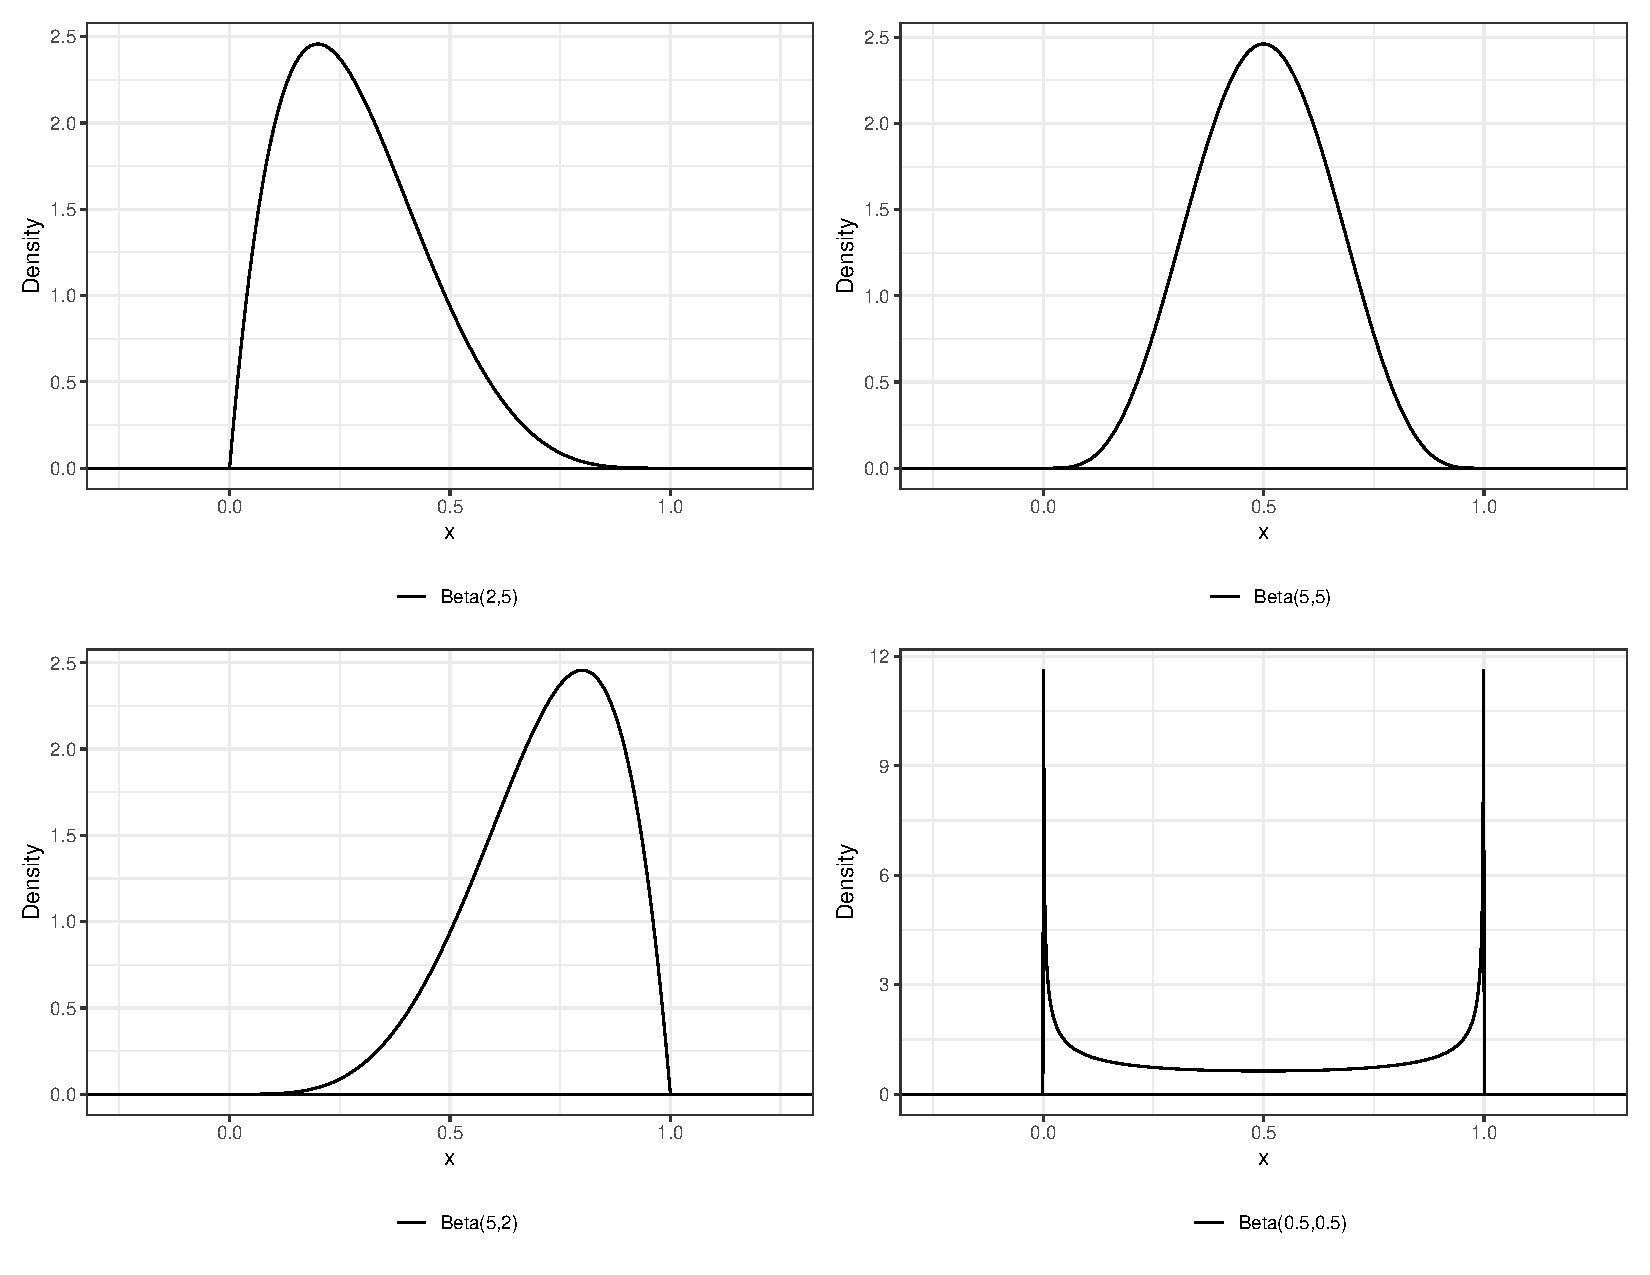
\includegraphics[width=\maxwidth]{figure/unnamed-chunk-5-1} 

}


\end{knitrout}
\caption{Population Distribution Plot by Case}
\label{plot1} 
\end{center}
\end{figure}




% latex table generated in R 4.4.2 by xtable 1.8-4 package
% Mon Mar 31 20:50:07 2025
\begin{table}[H]
\centering
\begingroup\small
\begin{tabular}{rrrrrr}
  \hline
Alpha & Beta & mean & variance & skewness & excess.kurtosis \\ 
  \hline
2.00 & 5.00 & 0.29 & 0.03 & 0.60 & -0.12 \\ 
  5.00 & 5.00 & 0.50 & 0.02 & -0.00 & -0.46 \\ 
  5.00 & 2.00 & 0.71 & 0.03 & -0.60 & -0.12 \\ 
  0.50 & 0.50 & 0.50 & 0.12 & -0.00 & -1.50 \\ 
   \hline
\end{tabular}
\endgroup
\caption{Moments Summary Table} 
\label{Table 2}
\end{table}



\begin{figure}[H]
\begin{center}
\begin{knitrout}
\definecolor{shadecolor}{rgb}{0.969, 0.969, 0.969}\color{fgcolor}

{\centering 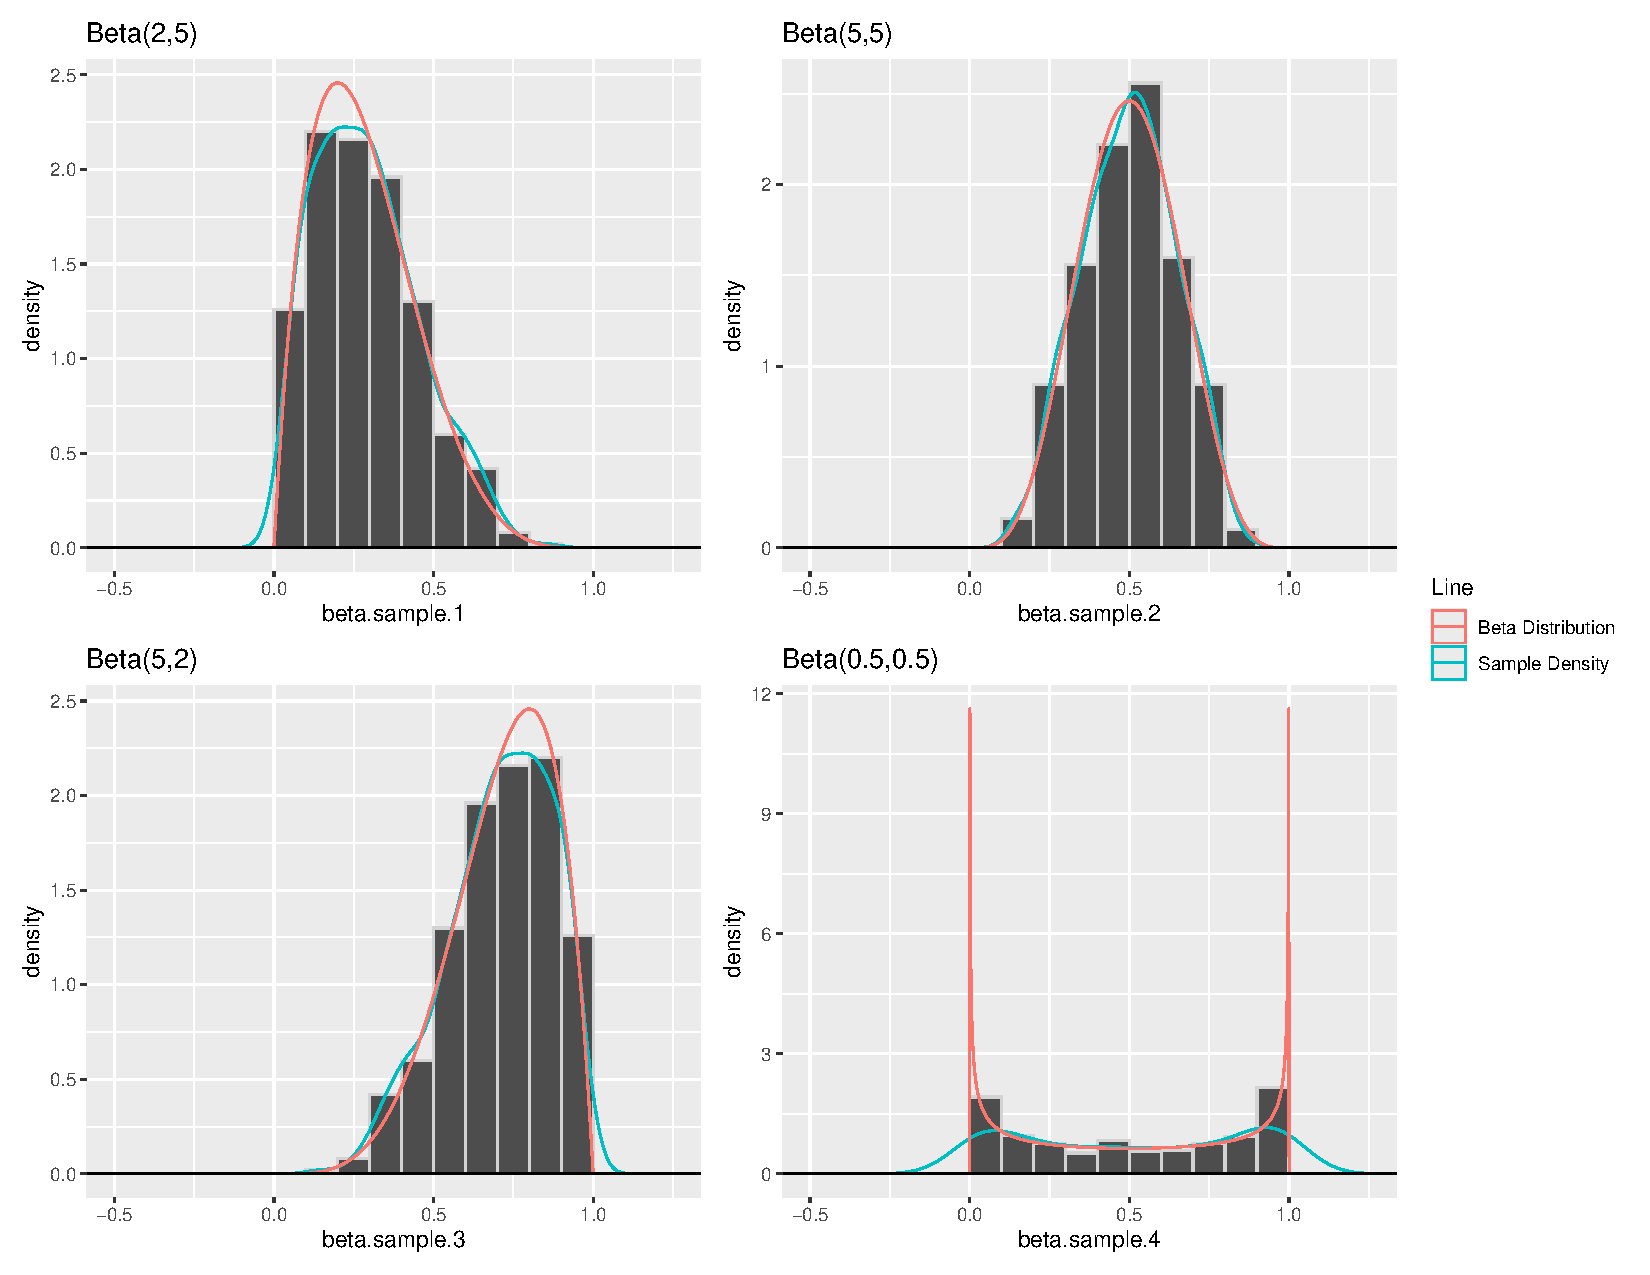
\includegraphics[width=\maxwidth]{figure/unnamed-chunk-8-1} 

}


\end{knitrout}
\caption{Sample Plot by Four Beta Distributions \citep{e1071}}
\label{plot2} 
\end{center}
\end{figure}

% latex table generated in R 4.4.2 by xtable 1.8-4 package
% Mon Mar 31 20:50:08 2025
\begin{table}[H]
\centering
\begingroup\small
\begin{tabular}{rrrrrr}
  \hline
Alpha & Beta & mean & variance & skewness & excess.kurtosis \\ 
  \hline
2.00 & 5.00 & 0.29 & 0.03 & 0.60 & -0.12 \\ 
  5.00 & 5.00 & 0.50 & 0.02 & -0.00 & -0.46 \\ 
  5.00 & 2.00 & 0.71 & 0.03 & -0.60 & -0.12 \\ 
  0.50 & 0.50 & 0.50 & 0.12 & -0.00 & -1.50 \\ 
   \hline
\end{tabular}
\endgroup
\caption{Sample Summary Table} 
\label{Table 3}
\end{table}



\begin{figure}[H]
\begin{center}
\begin{knitrout}
\definecolor{shadecolor}{rgb}{0.969, 0.969, 0.969}\color{fgcolor}

{\centering 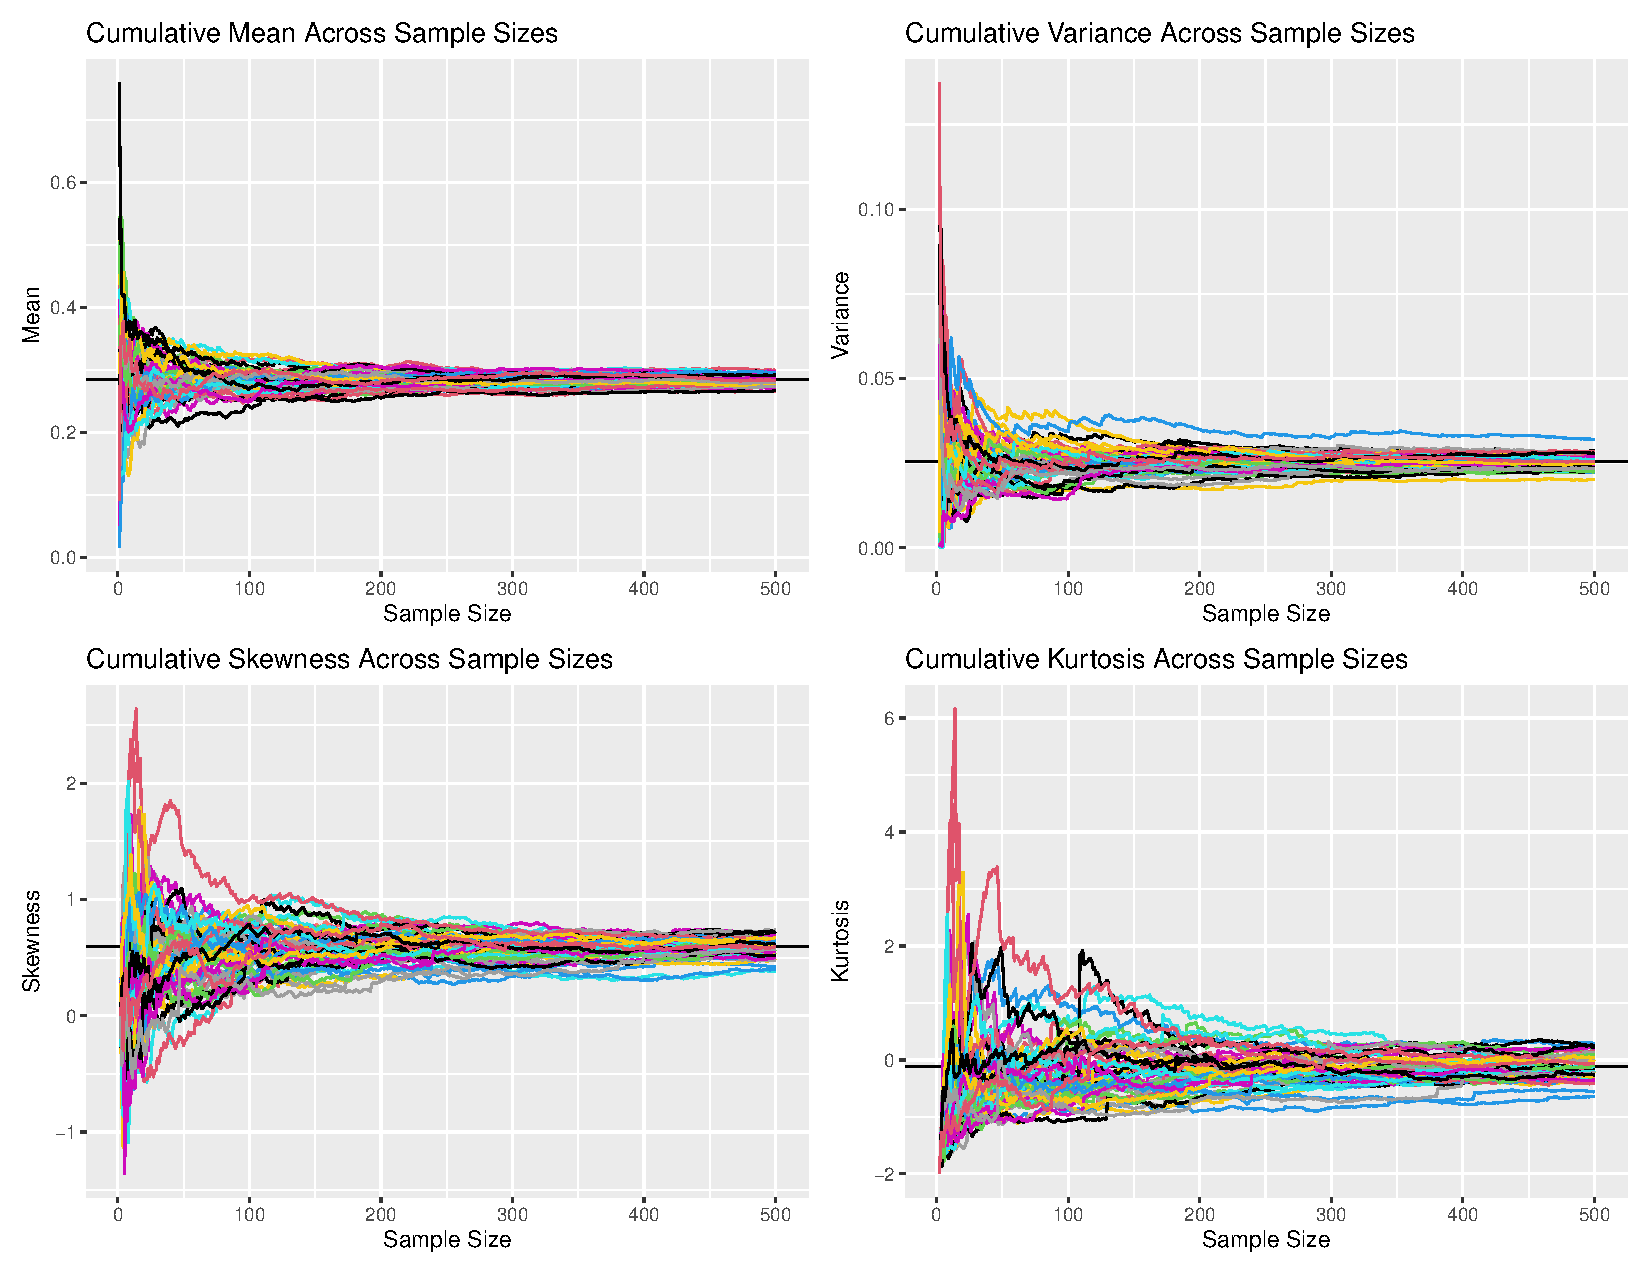
\includegraphics[width=\maxwidth]{figure/unnamed-chunk-10-1} 

}


\end{knitrout}
\caption{Cumulative Stats For Increasing Sample Sizes}
\label{plot3} 
\end{center}
\end{figure}


\begin{figure}[H]
\begin{center}
\begin{knitrout}
\definecolor{shadecolor}{rgb}{0.969, 0.969, 0.969}\color{fgcolor}

{\centering 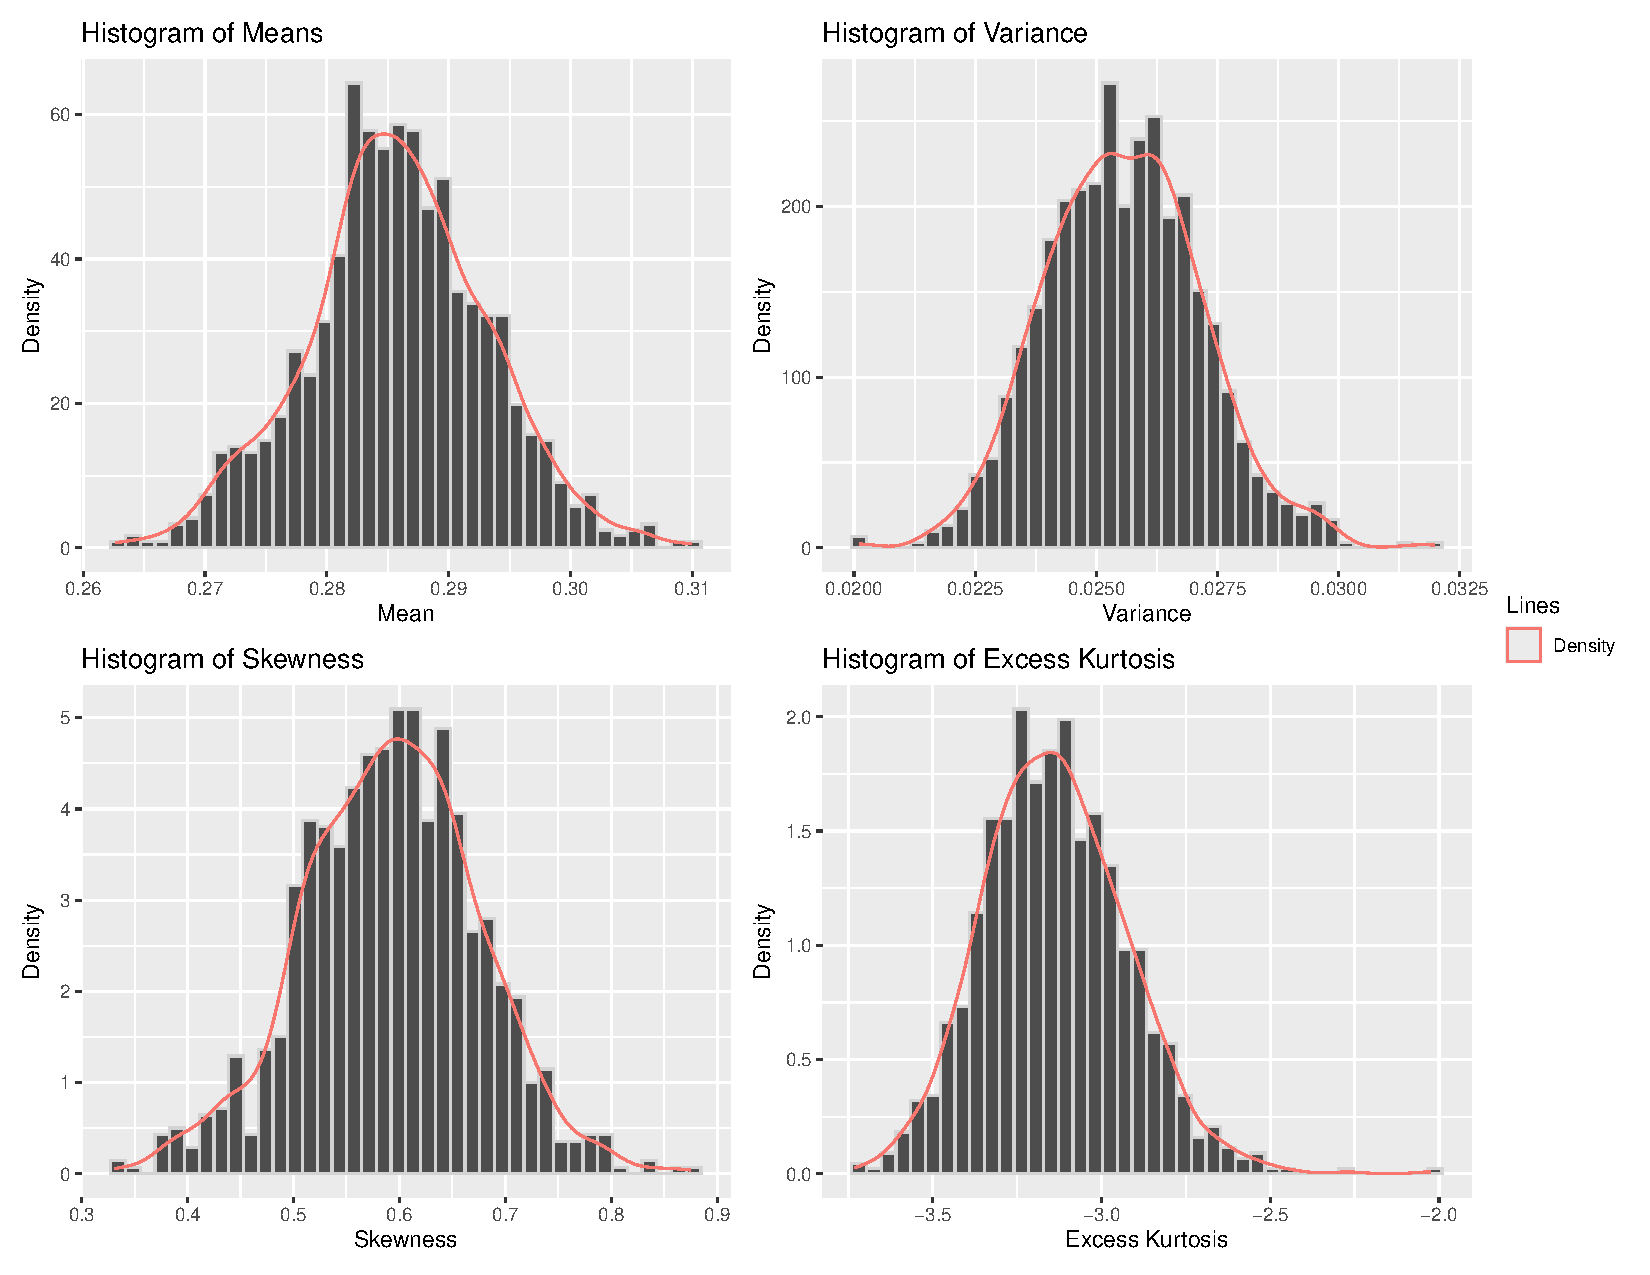
\includegraphics[width=\maxwidth]{figure/unnamed-chunk-11-1} 

}


\end{knitrout}
\caption{Histogram of Statistics}
\label{plot4} 
\end{center}
\end{figure}


\begin{figure}[H]
\begin{center}
\begin{knitrout}
\definecolor{shadecolor}{rgb}{0.969, 0.969, 0.969}\color{fgcolor}

{\centering 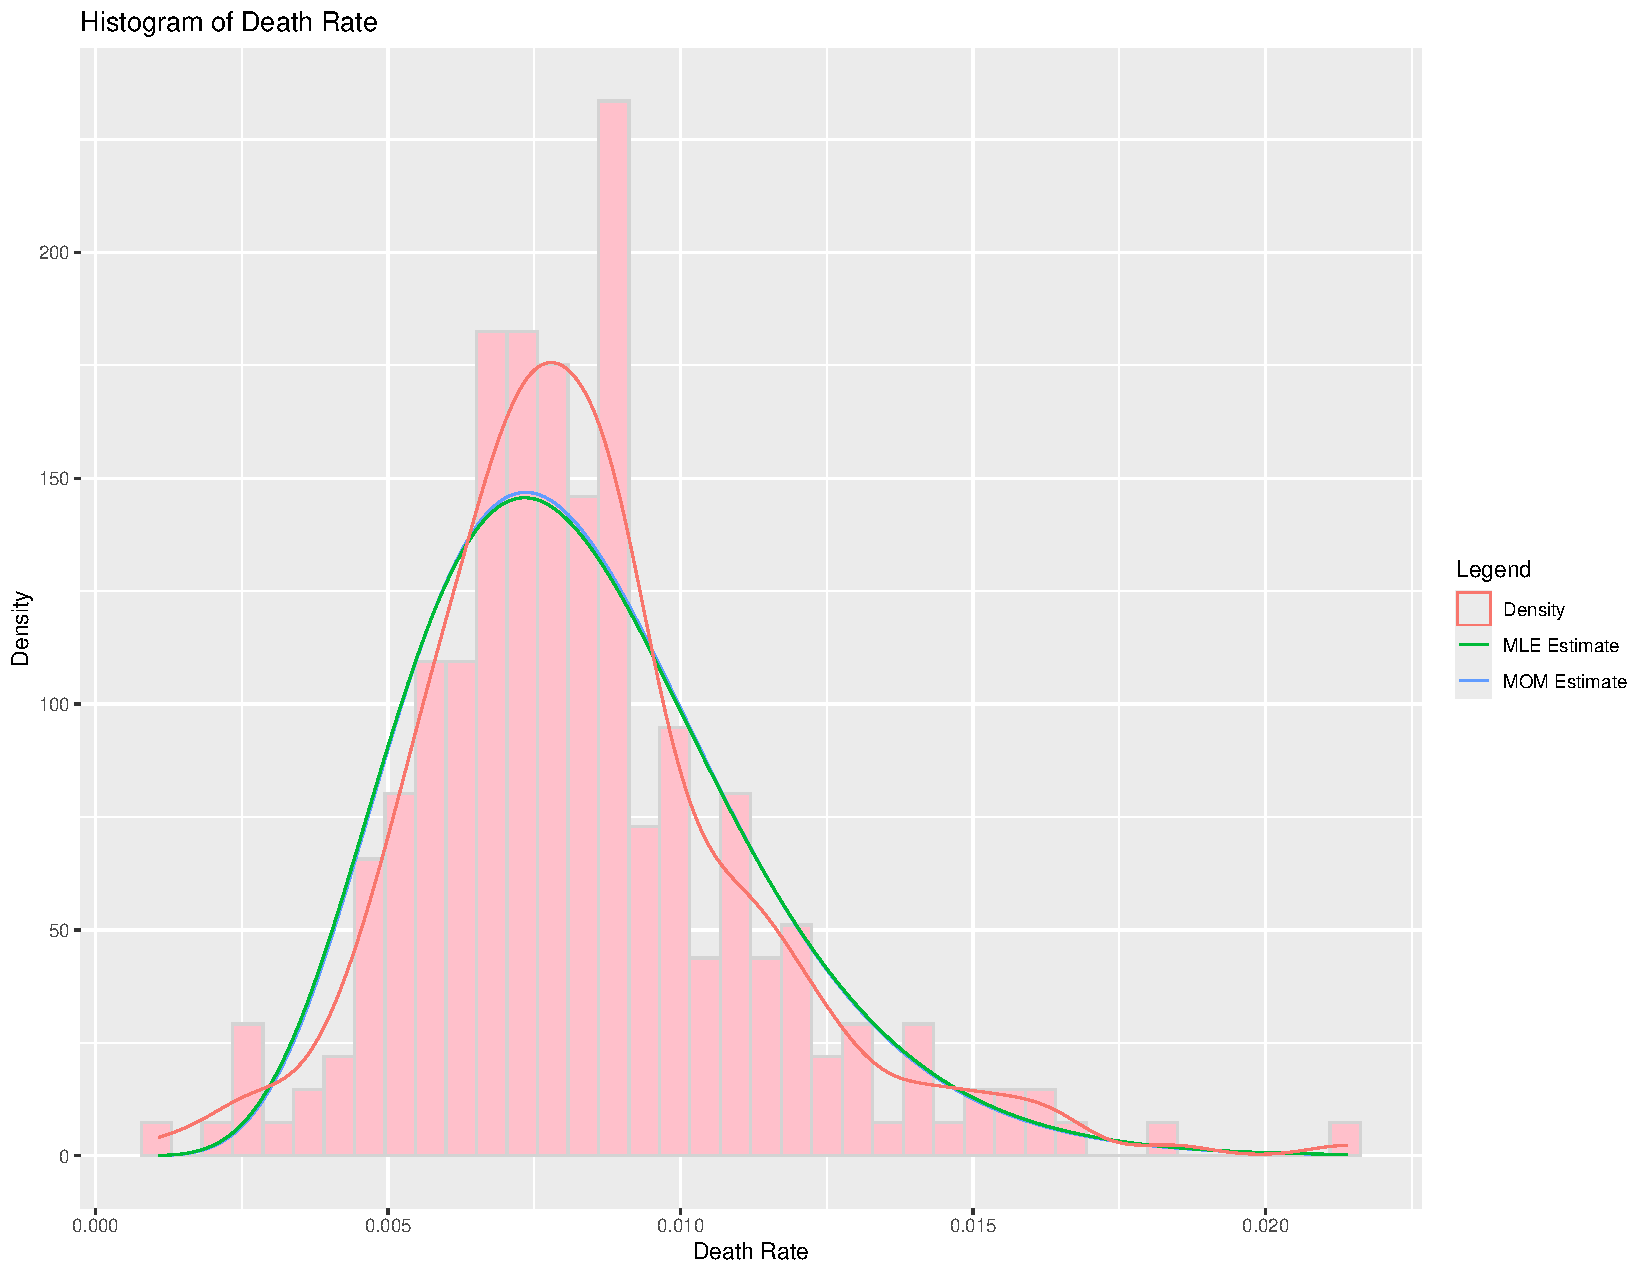
\includegraphics[width=\maxwidth]{figure/unnamed-chunk-12-1} 

}


\end{knitrout}
\caption{Histogram of Death Rate}
\label{plot5} 
\end{center}
\end{figure}


\begin{figure}[H]
\begin{center}
\begin{knitrout}
\definecolor{shadecolor}{rgb}{0.969, 0.969, 0.969}\color{fgcolor}

{\centering 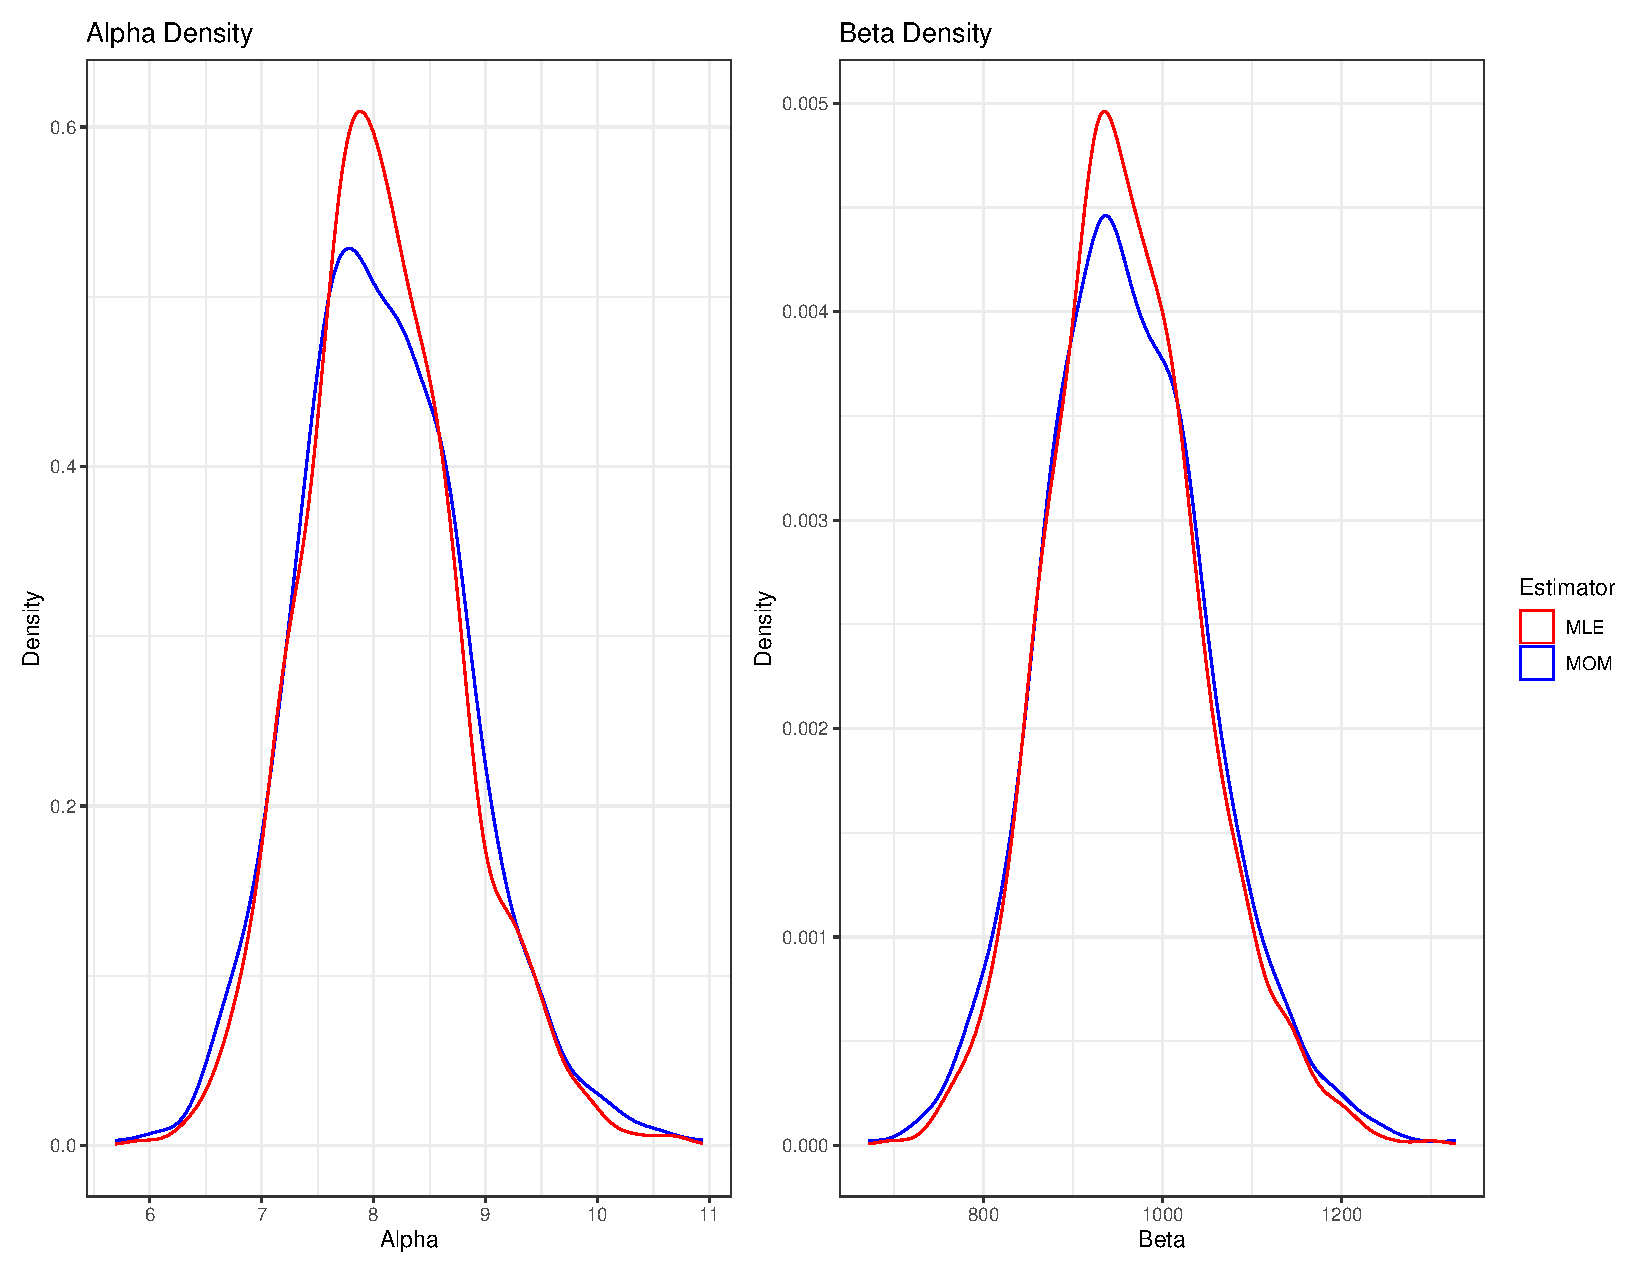
\includegraphics[width=\maxwidth]{figure/unnamed-chunk-13-1} 

}


\end{knitrout}
\caption{Density for MOM and MLE: Alpha and Beta Estimates}
\label{plot6} 
\end{center}
\end{figure}
% latex table generated in R 4.4.2 by xtable 1.8-4 package
% Mon Mar 31 20:50:13 2025
\begin{table}[H]
\centering
\begingroup\small
\begin{tabular}{lrrrrrr}
  \hline
Parameter & Bias\_MOM & Bias\_MLE & Precision\_MOM & Precision\_MLE & MSE\_MOM & MSE\_MLE \\ 
  \hline
Alpha & 0.08 & 0.07 & 1.83 & 2.13 & 0.55 & 0.47 \\ 
  Beta & 10.57 & 9.18 & 0.00 & 0.00 & 8303.00 & 7118.73 \\ 
   \hline
\end{tabular}
\endgroup
\caption{Summary for MLE and MOM} 
\label{Table 5}
\end{table}



\end{document}
